\documentclass[11pt]{article}
\usepackage[margin=1in]{geometry}
\usepackage{mathpazo}
\usepackage{amsmath,amssymb}
\usepackage{microtype}
\usepackage{booktabs}
\usepackage{graphicx}
\usepackage[dvipsnames]{xcolor}
\usepackage{tikz}
\usetikzlibrary{positioning,arrows.meta,calc,fit,backgrounds}
\usepackage[most]{tcolorbox}
\usepackage{enumitem}
\usepackage{listings}
\usepackage[font=small,labelfont=bf]{caption}
\usepackage{hyperref}
\hypersetup{colorlinks=true,linkcolor=MidnightBlue,citecolor=MidnightBlue,urlcolor=MidnightBlue}
\usepackage{cleveref}
\urlstyle{tt}
\def\UrlBreaks{\do\_\do/\do.}
\newcommand{\file}[1]{\nolinkurl{#1}}
\newcommand{\code}[1]{\texttt{#1}}
\newcommand{\mhh}{m_{hh}}
\newcommand{\bw}{\boldsymbol{\omega}}
\newcommand{\bp}{\boldsymbol{p}}
\newcommand{\bx}{\boldsymbol{x}}
\newcommand{\data}{\mathcal{D}}

\definecolor{trainable}{HTML}{1B6CA8}
\definecolor{physics}{HTML}{2E933C}
\definecolor{datac}{HTML}{7B4EA3}
\definecolor{warn}{HTML}{C0392B}

\newtcolorbox{keyidea}[1][]{enhanced,breakable,colback=physics!6,colframe=physics!70!black,
  fonttitle=\bfseries,title={#1},boxrule=0.6pt,arc=2pt,left=6pt,right=6pt}
\newtcolorbox{aside}[1][]{enhanced,breakable,colback=trainable!5,colframe=trainable!70!black,
  fonttitle=\bfseries,title={#1},boxrule=0.6pt,arc=2pt,left=6pt,right=6pt}
\newtcolorbox{assume}[1][]{enhanced,breakable,colback=datac!5,colframe=datac!70!black,
  fonttitle=\bfseries,title={#1},boxrule=0.6pt,arc=2pt,left=6pt,right=6pt}
\newtcolorbox{watch}[1][]{enhanced,breakable,colback=warn!5,colframe=warn!70!black,
  fonttitle=\bfseries,title={#1},boxrule=0.6pt,arc=2pt,left=6pt,right=6pt}
\setlist{itemsep=2pt,topsep=3pt}
\setlength{\emergencystretch}{3em}

\lstset{language=bash, basicstyle=\ttfamily\small, columns=fullflexible,
  keepspaces=true, commentstyle=\color{physics!70!black}\itshape,
  keywordstyle=\color{trainable!90!black}\bfseries, stringstyle=\color{datac},
  showstringspaces=false, frame=single, rulecolor=\color{gray!40},
  backgroundcolor=\color{gray!3}, xleftmargin=4pt, xrightmargin=4pt,
  aboveskip=6pt, belowskip=6pt}
\lstdefinestyle{sh}{language=bash, keywordstyle=\color{black}, commentstyle=\color{black}}

\title{\textbf{Running the \texttt{dihiggs} notebooks on the RTX 5090}\\[4pt]
\large A short manual: long runs that survive a broken connection,\\ with a \texttt{tmux} cheat sheet}
\date{October 31, 2026 (first version October 30)}

\begin{document}
\maketitle

\begin{abstract}
\noindent
The BNN and ensemble notebooks run for an hour or more on the 5090, reached from a laptop
by \code{ssh}. This note explains which parts of the set-up live where, what survives a
closed browser tab or a broken connection, and how to start, watch, interrupt, resume and
collect a run. Names in angle brackets, such as \code{<user>@<host>}, stand for your own
values. The conda environment on the 5090 is \code{ml}; the repository is
\file{~/Projects/workbench/dihiggs} there and \file{~/Projects/Tutorials/GitHub/dihiggs} on the Mac.
\end{abstract}

\begin{keyidea}[The one rule]
Everything that must keep running is started, directly or indirectly, inside \code{tmux}
on the 5090. Then the laptop, the browser and the \code{ssh} connection can all go away
without stopping it.
\end{keyidea}

% ===========================================================================
\section{What runs where}

\begin{figure}[h]
\centering
\resizebox{\textwidth}{!}{%
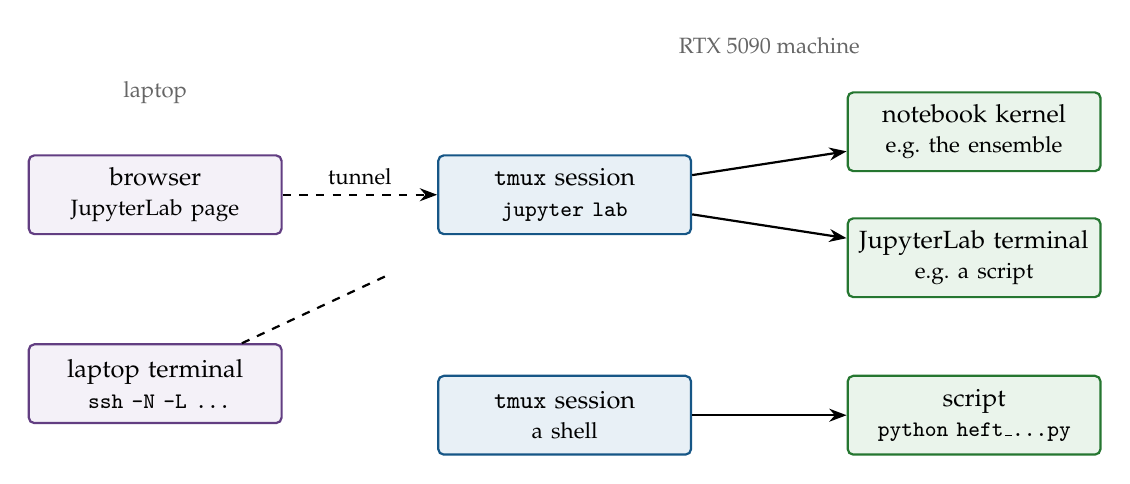
\begin{tikzpicture}[
  font=\small, >={Stealth[length=2.2mm]},
  box/.style={draw, rounded corners=2pt, thick, align=center, inner sep=3pt,
              minimum height=10mm, text width=30mm},
  lap/.style={box, fill=datac!8, draw=datac!80!black},
  gpu/.style={box, fill=trainable!10, draw=trainable!80!black},
  job/.style={box, fill=physics!10, draw=physics!80!black},
]
\node[lap] (browser) at (0, 1.2) {browser\\\footnotesize JupyterLab page};
\node[lap] (term)    at (0, -1.2) {laptop terminal\\\footnotesize \code{ssh -N -L ...}};
\node[gpu] (tmux1)   at (5.2, 1.2) {\code{tmux} session\\\footnotesize \code{jupyter lab}};
\node[gpu] (tmux2)   at (5.2, -1.6) {\code{tmux} session\\\footnotesize a shell};
\node[job] (kern)    at (10.4, 2.0) {notebook kernel\\\footnotesize e.g.\ the ensemble};
\node[job] (jterm)   at (10.4, 0.4) {JupyterLab terminal\\\footnotesize e.g.\ a script};
\node[job] (script)  at (10.4, -1.6) {script\\\footnotesize \code{python heft\_...py}};
\draw[->, thick, dashed] (browser) -- node[above, font=\footnotesize]{tunnel} (tmux1);
\draw[thick, dashed] (term) -- (3.0, 0.2);
\draw[->, thick] (tmux1) -- (kern);
\draw[->, thick] (tmux1) -- (jterm);
\draw[->, thick] (tmux2) -- (script);
\node[font=\footnotesize, text=black!60] at (0, 2.5) {laptop};
\node[font=\footnotesize, text=black!60] at (7.8, 3.1) {RTX 5090 machine};
\end{tikzpicture}}
\caption{Purple: on the laptop; they may disappear at any time. Blue and green: on the
5090. Kernels and JupyterLab terminals belong to the Jupyter server; scripts started in
their own \code{tmux} session depend on nothing else.}
\label{fig:where}
\end{figure}

\begin{center}
\small
\begin{tabular}{p{0.46\textwidth}cc}
\toprule
event & the run in Jupyter & a script in \code{tmux}\\
\midrule
close the browser tab or the browser & continues & continues\\
break the tunnel, close the laptop, lose the network & continues & continues\\
JupyterLab: close a notebook or terminal \emph{tab} & continues & continues\\
JupyterLab: \textbf{Shut Down} kernel/terminal, \textbf{File $\to$ Shut Down} & \textbf{stops} & continues\\
\code{Ctrl-c} in the \code{tmux} pane running \code{jupyter lab} & \textbf{stops} & continues\\
\code{Ctrl-c} in the \code{tmux} pane running the script & continues & \textbf{stops}\\
the 5090 reboots & \textbf{stops} & \textbf{stops}\\
\bottomrule
\end{tabular}
\end{center}

\noindent While no browser is connected, the kernel's printed output is not recorded in
the notebook. The computation and every file it writes (run folders, traces, figures) are
unaffected.


% ===========================================================================
\section{Who owns a process: the rule behind everything}
\label{sec:owner}

Every process on the 5090 has a parent, and what happens to it when you disconnect depends
on that parent. When an \code{ssh} session ends, normally or because the connection drops,
the system sends its shell a \emph{hang-up} signal (SIGHUP), and the shell passes it on to
the jobs it started, which then stop. A process survives if its parent does not hang up, or
if it has been told to ignore the signal.

\begin{center}
\small
\begin{tabular}{p{0.36\textwidth}p{0.30\textwidth}c}
\toprule
started from & belongs to & survives logout?\\
\midrule
a notebook in JupyterLab & the Jupyter server (in \code{tmux}) & yes\\
a JupyterLab terminal & the Jupyter server (in \code{tmux}) & yes\\
a login shell, \code{command \&} & your login session & \textbf{no}\\
a login shell, \code{nohup command \&} & nobody who will hang up & yes\\
a shell inside \code{tmux} & the \code{tmux} server & yes\\
\bottomrule
\end{tabular}
\end{center}

\noindent The browser page on the laptop is only a window onto JupyterLab, and the tunnel
only the line to it: closing either touches nothing on the 5090.

\paragraph{\code{nohup}.} \code{nohup bash run.sh > /dev/null 2>\&1 \&} starts the script in
the background, immune to the hang-up signal. \code{> /dev/null 2>\&1} discards what the
script prints to the terminal; if the script itself writes a log (with \code{tee}), nothing
is lost. Use it for a one-off job from a login shell. The disadvantage: you cannot come
back to the job's terminal later; you can only read its log.

% ===========================================================================
\section{The \texttt{tmux} programming model}
\label{sec:tmux}

\begin{figure}[h]
\centering
\resizebox{\textwidth}{!}{%
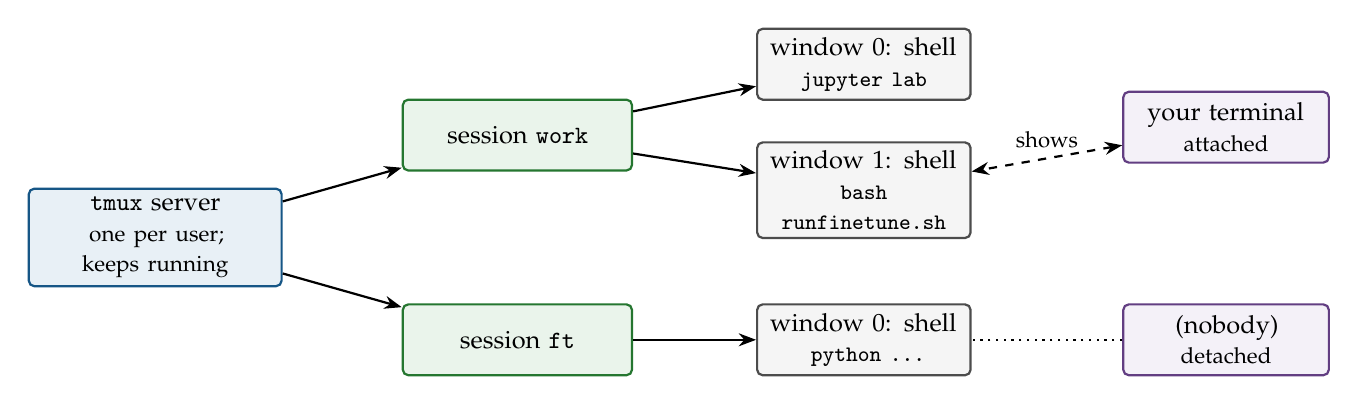
\begin{tikzpicture}[
  font=\small, >={Stealth[length=2.2mm]},
  box/.style={draw, rounded corners=2pt, thick, align=center, inner sep=3pt,
              minimum height=9mm, text width=27mm},
  srv/.style={box, fill=trainable!10, draw=trainable!80!black, text width=30mm},
  ses/.style={box, fill=physics!10, draw=physics!80!black},
  win/.style={box, fill=gray!8, draw=gray!60!black, text width=25mm},
  cli/.style={box, fill=datac!8, draw=datac!80!black, text width=24mm},
]
\node[srv] (server) at (0, 0) {\code{tmux} server\\\footnotesize one per user; keeps running};
\node[ses] (s1) at (4.6, 1.3) {session \code{work}};
\node[ses] (s2) at (4.6, -1.3) {session \code{ft}};
\node[win] (w0) at (9.0, 2.2) {window 0: shell\\\footnotesize \code{jupyter lab}};
\node[win] (w1) at (9.0, 0.6) {window 1: shell\\\footnotesize \code{bash runfinetune.sh}};
\node[win] (w2) at (9.0, -1.3) {window 0: shell\\\footnotesize \code{python ...}};
\node[cli] (c1) at (13.6, 1.4) {your terminal\\\footnotesize attached};
\node[cli] (c2) at (13.6, -1.3) {(nobody)\\\footnotesize detached};
\draw[->, thick] (server) -- (s1);
\draw[->, thick] (server) -- (s2);
\draw[->, thick] (s1) -- (w0);
\draw[->, thick] (s1) -- (w1);
\draw[->, thick] (s2) -- (w2);
\draw[<->, thick, dashed] (c1) -- node[above, font=\footnotesize]{shows} (w1);
\draw[thick, dotted] (c2) -- (w2);
\end{tikzpicture}}
\caption{\code{tmux}'s structure. The server owns sessions, sessions own windows, and each
window runs a shell, in which your programs run. A terminal \emph{attached} to a session
shows one of its windows; \emph{detaching} disconnects the terminal and leaves everything
running.}
\label{fig:tmux}
\end{figure}

\begin{itemize}
  \item \textbf{The server} starts automatically with the first \code{tmux} command and runs
    until its last session ends (or the machine reboots). It is the parent of every shell
    in every window, which is why those shells, and the programs they run, survive your
    logging out.
  \item \textbf{A session} is a named group of windows, e.g.\ \code{work}. You attach to a
    session from any terminal (an \code{ssh} login today, another one tomorrow) and detach
    from it at will; it does not care which terminal, if any, is looking at it.
  \item \textbf{A window} is one full-screen shell, numbered 0, 1, 2, \ldots and shown in the
    status bar at the bottom. Use one window per job: e.g.\ window 0 for
    \code{jupyter lab}, window 1 for a fine-tune, window 2 for watching logs.
  \item \textbf{A pane} is a window split into parts, each with its own shell. Optional;
    handy for watching \code{nvidia-smi} beside a log.
  \item \textbf{The prefix key.} \code{tmux} commands typed \emph{inside} a session start with
    the prefix \code{Ctrl-b}: press and release \code{Ctrl-b}, then the command key. For
    example \code{Ctrl-b} then \code{d} detaches.
  \item \textbf{Ending things.} \code{exit} in a window's shell closes that window (and the
    session, when its last window closes). \code{Ctrl-c} stops the program running in the
    current window, not \code{tmux}. Neither should ever be used in the window running
    \code{jupyter lab} unless you mean to stop JupyterLab.
\end{itemize}

\begin{keyidea}[Adding a job to a session that is already running]
Attach (\code{tmux attach -t work}), open a new window (\code{Ctrl-b c}), start the job
there with no \code{\&} or \code{nohup} (the window's shell belongs to \code{tmux}), and detach
(\code{Ctrl-b d}). The new job and everything already running continue.
\end{keyidea}

% ===========================================================================
\section{\texttt{tmux} cheat sheet}
\label{sec:cheat}

\paragraph{Shell commands} (typed at a prompt, outside or inside \code{tmux}).
\begin{center}
\small
\begin{tabular}{p{0.38\textwidth}p{0.55\textwidth}}
\toprule
command & what it does\\
\midrule
\code{tmux new -s work} & start a new session called \code{work} and attach to it\\
\code{tmux ls} & list the sessions\\
\code{tmux attach -t work} & attach to session \code{work}\\
\code{tmux attach} & attach to the most recent session\\
\code{tmux new-window -t work} & add a window to \code{work} without attaching\\
\code{tmux kill-session -t work} & end a session and everything running in it\\
\bottomrule
\end{tabular}
\end{center}

\paragraph{Keys inside a session} (press \code{Ctrl-b}, release, then the key).
\begin{center}
\small
\begin{tabular}{p{0.20\textwidth}p{0.73\textwidth}}
\toprule
\code{Ctrl-b}, then & what it does\\
\midrule
\code{d} & detach: leave everything running and return to the plain shell\\
\code{c} & create a new window\\
\code{n} / \code{p} & next / previous window\\
\code{0} \ldots\ \code{9} & go to window 0 \ldots\ 9\\
\code{w} & choose a window (or session) from a list\\
\code{,} & rename the current window (e.g.\ \code{jupyter}, \code{finetune})\\
\code{\%} / \code{"} & split the window into two panes, side by side / one above the other\\
\code{o} & move to the next pane\\
\code{x} & close the current pane (asks for confirmation)\\
\code{[} & scroll mode: look back through the output with the arrow keys or
  PageUp/PageDown; \code{q} leaves it\\
\code{?} & list all key bindings\\
\bottomrule
\end{tabular}
\end{center}

\paragraph{A typical day.}
\begin{lstlisting}[style=sh]
ssh <user>@<host>
tmux ls
tmux attach -t work
\end{lstlisting}
\noindent Then \code{Ctrl-b w} to see the windows, \code{Ctrl-b c} for a new one, run the job,
\code{Ctrl-b d} to leave. If \code{tmux ls} says there is no server, nothing is running in
\code{tmux}: start with \code{tmux new -s work}.

\begin{watch}[Three slips to avoid]
\begin{enumerate}
  \item Typing a new job into the window running \code{jupyter lab}: that window is busy, and
    \code{Ctrl-c} there stops JupyterLab. Open a new window instead.
  \item Starting \code{tmux} inside \code{tmux} (running \code{tmux new} from a window of an
    attached session): \code{tmux} warns about nesting; use \code{Ctrl-b c} for another
    window instead.
  \item Closing the laptop's terminal \emph{without} detaching is harmless: the session
    simply becomes detached. But \code{exit} typed in a window closes that window, and
    whatever it was running stops.
\end{enumerate}
\end{watch}

% ===========================================================================
\section{Updating the code first}

On the Mac, commit and push; on the 5090, pull:
\begin{lstlisting}[style=sh]
cd ~/Projects/Tutorials/GitHub/dihiggs
git push
\end{lstlisting}
\begin{lstlisting}[style=sh]
cd ~/Projects/workbench/dihiggs
git pull
\end{lstlisting}
Then restart any Jupyter kernel that imports \code{dihiggs}, so that it loads the new
modules. If \code{git pull} refuses because a notebook was edited on the 5090 (for example
its switches), discard that edit and pull again, then re-enter the switches:
\begin{lstlisting}[style=sh]
git checkout code/heft_train_bnn.ipynb
git pull
\end{lstlisting}
A quick check that the 5090 has the new \file{hmc.py}: a BNN run prints, at the start, a
line beginning \code{warm-up: step size only for iterations 1-75}.

% ===========================================================================
\section{Recipe A: a script in its own \texttt{tmux} session (most robust)}

\begin{enumerate}
  \item Set the switches in the notebook (in JupyterLab, or any editor) and save it.
  \item On the 5090, start a named \code{tmux} session (or, if one is already running,
    attach to it and open a new window with \code{Ctrl-b c}; \cref{sec:tmux}) and go to the
    code folder:
\begin{lstlisting}[style=sh]
tmux new -s bnn
conda activate ml
cd ~/Projects/workbench/dihiggs/code
\end{lstlisting}
  \item Convert the notebook to a script, and run it:
\begin{lstlisting}[style=sh]
jupyter nbconvert --to python heft_train_bnn.ipynb
MPLBACKEND=Agg python heft_train_bnn.py 2>&1 | tee bnn_run.log
\end{lstlisting}
    \code{--to python} always writes a \file{.py} file (\code{--to script} takes the
    extension from the notebook's metadata, and for a notebook never saved in Jupyter may
    write a \file{.txt} file instead). \code{MPLBACKEND=Agg} makes matplotlib write figures to files instead of opening
    windows; \code{tee} shows the output and also keeps it in \file{bnn_run.log}.
  \item Detach: press \code{Ctrl-b}, then \code{d}. You may now log out.
  \item Later, reattach with
\begin{lstlisting}[style=sh]
tmux attach -t bnn
\end{lstlisting}
\end{enumerate}
\noindent The same works for \file{heft_train_ensemble.ipynb} (choose another session
name, e.g.\ \code{ens}, and another log file). Re-run the \code{nbconvert} line whenever
the notebook changes, or the script will run the old switches.

% ===========================================================================
\section{Recipe B: JupyterLab through an \texttt{ssh} tunnel}

\begin{enumerate}
  \item On the 5090, start the Jupyter server inside \code{tmux}, then detach
    (\code{Ctrl-b}, \code{d}):
\begin{lstlisting}[style=sh]
tmux new -s jupyter
conda activate ml
cd ~/Projects/workbench/dihiggs
jupyter lab --no-browser --port <port>
\end{lstlisting}
    Note the URL with its token that it prints.
  \item On the laptop, open the tunnel in a terminal of its own, and leave it open:
\begin{lstlisting}[style=sh]
ssh -N -L <port>:localhost:<port> <user>@<host>
\end{lstlisting}
    Then open \code{http://localhost:<port>} (with the token) in the browser.
  \item Run the notebook as usual, or open a JupyterLab terminal and run Recipe A's
    script commands there (step 3).
  \item To leave: close the browser tab, then press \code{Ctrl-c} in the tunnel's
    terminal (or close it). Never use the \textbf{Shut Down} entries of JupyterLab for a
    run you want to keep.
  \item To come back: open the tunnel again and reload the page.
\end{enumerate}

\begin{watch}[A script started in a JupyterLab terminal]
It runs on the 5090 and survives a closed tab and a broken tunnel, but it belongs to the
Jupyter server: if the server stops, so does the script. For long runs, Recipe A is safer.
\end{watch}

% ===========================================================================
\section{Watching a run}

From any \code{ssh} session on the 5090, in \file{~/Projects/workbench/dihiggs/code}: the
script's output so far, the BNN trace (one line per iteration), the ensemble summary (one
line per member), the GPU, and the running \code{tmux} sessions:
\begin{lstlisting}[style=sh]
cd ~/Projects/workbench/dihiggs/code
tail -n 30 bnn_run.log
tail -f runs/BNN_poisson/dihiggs_hmc_trace.csv
cat runs/ENS_bootstrap/ensemble.csv
nvidia-smi
tmux ls
\end{lstlisting}
\noindent \code{tail -f} keeps printing new lines; \code{Ctrl-c} stops the watching, not
the run.

% ===========================================================================
\section{Interrupting and resuming}

\begin{itemize}
  \item \textbf{BNN.} Stop a run with \code{Ctrl-c} in its \code{tmux} pane, or
    \textbf{Kernel $\to$ Interrupt} in JupyterLab. The sampler then saves a checkpoint at
    the last complete iteration (it also saves one every few minutes, in case of a crash).
    To continue, set \code{RESUME = True}, keep the other switches, save, and run again
    (for Recipe A, re-run the \code{nbconvert} line first). The result is identical to an
    uninterrupted run. A larger \code{N\_SAMPLES} extends a finished run.
  \item \textbf{Ensemble.} Members already finished are skipped, so just run the notebook
    again; at most the member in progress is lost.
  \item \textbf{Before resuming,} make sure the old run has really stopped (\code{tmux ls},
    \code{nvidia-smi}): two processes writing to the same run folder would corrupt it.
\end{itemize}

% ===========================================================================
\section{Several jobs on one GPU}

\code{HEFTNet} is small: each job needs about 0.5--1 GB of the 5090's 32 GB, and much of its
time is Python overhead, so two or three jobs can share the GPU, each running somewhat
slower. Check \code{nvidia-smi}: if the utilisation is already near 100\%, another job
mainly slows the others down. Each job also keeps about one CPU core busy. Two copies of
the ensemble notebook can train different members at once, with disjoint
\code{MEMBERS} ranges such as \code{range(0, 10)} and \code{range(10, 20)}.

% ===========================================================================
\section{Bringing the results back to the Mac}

On the 5090, pack the run folder; on the Mac, copy it into \file{code/runs/}:
\begin{lstlisting}[style=sh]
cd ~/Projects/workbench/dihiggs/code/runs
tar czf BNN_poisson.tar.gz BNN_poisson
\end{lstlisting}
\begin{lstlisting}[style=sh]
cd ~/Projects/Tutorials/GitHub/dihiggs/code/runs
scp <user>@<host>:Projects/workbench/dihiggs/code/runs/BNN_poisson.tar.gz .
tar xzf BNN_poisson.tar.gz
\end{lstlisting}

\begin{watch}[Run folders are overwritten]
A new BNN run with the same likelihood writes into the same folder,
\file{runs/BNN_<likelihood>}, and replaces the previous run. Rename the old folder first
(e.g.\ \file{BNN_poisson} $\to$ \file{BNN_poisson3}), on the 5090 before starting, and on
the Mac before unpacking.
\end{watch}

\end{document}
